\subsection[]{Dimostrare l’espressione
\[
	\frac{dt}{dt'}=1-\hat{n}\bs{\beta}
.\] 
dove t e t’ sono il tempo di osservazione ed il tempo ‘ritardato’, rispettivamente.}
\label{sec:3.b.1}
Si prenda una carica che si muove con la legge oraria $\bs{s}\left( t \right) $ e velocità $\bs{\beta}$, sfruttando la definizione di tempo ritardato: \[
	t=t_{\text{rit}} + \left| \bs{r}- \bs{s}\left( t_{\text{rit}} \right)  \right|/c 
.\]
Possiamo differenziare: \[
	\frac{\mbox{d} t}{\mbox{d} t_{\text{rit}}} = 1- \frac{\left( \bs{r}-\bs{s}\left( t_{\text{rit}} \right) \right)\cdot \frac{\mbox{d} \bs{s}\left( t_{\text{rit}} \right) }{\mbox{d} t_{\text{rit}}} }{\left| \bs{r}-\bs{s}\left( t_{\text{rit}} \right)  \right|c }=\left.1-\hat{n}\cdot \bs{\beta}\right|_{\text{rit}}
.\] 
\subsection[]{Date le definizioni ‘standard’ delle variabili $\hat{n}, \bs{\beta}, \bs{R}, \bs{r}, \bs{r}', t, t'$ , dimostrare le seguenti relazioni:
} \label{sec:3.b.2}
\begin{align*}
&1) \ \frac{\mbox{d} \bs{R}}{\mbox{d} t'} = -\bs{\beta}c 					&2)& \ \frac{\mbox{d}R}{\mbox{d}t'}=-\hat{n}\cdot\bs{\beta}c\\
& & &\\
&3) \ \frac{\mbox{d}\left(\bs{R}\cdot\bs{\beta}\right)}{\mbox{d}t'}=-\beta c+\bs{R}\cdot\bs{\beta}	&4)& \ \nabla\bs{R}=\frac{\hat{n}}{\left(1-\hat{n}\bs{\beta}\right)}\\
& & &\\
&5) \ \nabla t' = \frac{-\hat{n}/c}{1-\hat{n}\bs{\beta}}
.\end{align*}
Si ha che $\bs{r}$ e $t$ sono il punto e l'istante in cui si osservano i campi , $\bs{r}'$ la posizione delle sorgenti. $t'$ è il tempo ritardato definito da : \[
	c\left( t-t' \right) =\left| \bs{r}- \bs{r}'\left( t' \right)  \right| 
.\] 
Si ha inoltre che \[
	\bs{R}= \bs{r}-\bs{r}'\left( t' \right) 
.\]
Mentre $\hat{n} = \bs{R} /R$ e $\bs{\beta}=\dot{\bs{r}}' /c$. Possiamo inoltre derivare $\bs{R}$ rispetto al tempo ritardato per ottenere una delle relazioni: \[
	\frac{\mbox{d} \bs{R}}{\mbox{d} t'} = -\dot{\bs{r}}'=-\bs{\beta}c
.\] 
Facciamo quindi lo stesso con $R$ : \[
	\frac{\mbox{d} R}{\mbox{d} t'} = \frac{\mbox{d} \left| \bs{r}-\bs{r}' \right| }{\mbox{d} t'} = 
	\frac{\bs{R}}{R}\cdot \frac{\mbox{d} \bs{R}}{\mbox{d} t'}= - \hat{n}\cdot \bs{\beta}c
.\] 
E con il prodotto $\bs{R}\cdot \bs{\beta}$ : \[
	\frac{\mbox{d} \left( \bs{R}\cdot \bs{\beta} \right) }{\mbox{d} t'} = \bs{\beta}\cdot \frac{\mbox{d} \bs{R}}{\mbox{d} t'} + \bs{R}\frac{\mbox{d} \bs{\beta}}{\mbox{d} t'} = -\beta^2c + \bs{R}\cdot \dot{\bs{\beta}} 	
.\]
Dalla definizione di tempo ritardato si ha una utile relazione tra $\nabla t'$ e $\nabla R$ : \[
	-c\nabla t' = \nabla R 
.\] 
È necessario calcolare solo $\nabla t'$ per avere anche l'altra quantità:
\begin{align*}
	-c\nabla t' &= \nabla \left| \bs{r}-\bs{r}'\left( t' \right)  \right| =\\
		    &= \hat{x}_{i} \frac{\partial }{\partial x_{i} } \sqrt{\sum_{j=1}^{3} \left( r_{j}-r'_{j}\left( t' \right)  \right)^2 }=\\
		    &= \frac{\hat{x}_{i}}{2R} \frac{\partial }{\partial x_{i}} \sum_{j=1}^{3} \left( r_{j}-r'_{j}\left( t' \right)  \right) ^2 = \\
		    &= \frac{\hat{x}_{i}}{R} \sum_{j=1}^{3} \left( r_{j}-r'_{j}\left( t' \right)  \right)
		    \left( \delta_{ij}-c \beta_{j}\left( t' \right) \frac{\partial t'}{\partial x_{i}}  \right) =\\
		    &= \hat{n}- c \hat{n}\cdot \bs{\beta} \nabla t' 
.\end{align*}
Se ne conclude che : \[
	\nabla t'=-\frac{\hat{n} /c}{1-\hat{n}\cdot \bs{\beta}}
.\] 

\subsection[]{Calcolare la distribuzione in potenza in funzione dell’angolo di emissione per una carica accelerata in moto non relativistico.}
\label{sec:3.b.3}
Si parte dal campo generato da una carica in moto :
\[
	\bs{E}\left( \bs{x},t \right) = q \left[ \frac{\hat{n}-\bs{\beta}}{\gamma^2\left( 1-\hat{n}\cdot \bs{\beta} \right)^3 R^2 } \right]_{\text{rit}}+
	\frac{q}{c} \left[ \frac{\hat{n}\wedge \left[ \left( \hat{n}-\bs{\beta} \right) \wedge \dot{\bs{\beta}}  \right] }
	{\left( 1-\hat{n}\cdot \bs{\beta} \right)^3 R}  \right]_{\text{rit}} 
.\] \label{eq:L-W} 
Dove le quantità sono quelle definite nella domanda precedente. Si trascura adesso il campo a decrescsenza rapida e si considera solo il campo di radiazione approssimandolo al caso non relativistico:
\[
	\bs{E}_{\text{rad}}\left( \bs{x},t \right)= \frac{q}{c} \left[ \frac{\hat{n}\wedge \left[ \left( \hat{n}-\bs{\beta} \right) \wedge \dot{\bs{\beta}}  \right] }
	{\left( 1-\hat{n}\cdot \bs{\beta} \right)^3 R}  \right]_{\text{rit}}  \approx \frac{q}{c} \left[ \frac{\hat{n}\wedge \left( \hat{n}\wedge \dot{\bs{\beta}}\right)}{R} \right]_{\text{rit}} 
.\] 
L'approssimazione si ottiene raggruppando un $\hat{n}$ al numeratore. IL vettore di Poynting quindi è:
\[
	\bs{S}= \frac{c}{4 \pi} \left| \bs{E}_{\text{rad}} \right| ^2 \hat{n}=\frac{q^2}{4\pi c} 
	\left| \frac{\hat{n}\wedge \left( \hat{n}\wedge  \dot{\bs{\beta}}\right)}{R} \right|^2
.\] 
Dove si è anche trascurato il termine $\bs{\beta}$ rispetto al ternine $\hat{n}$ perchè discutiamo il caso  non relativistico. Andando adesso in un sistema di riferimento in cui $\theta$ è l'angolo tra la accelerazione della particella e la direzione di osservazione si ha:
\[
	\bs{S}= \frac{q^2}{4\pi R^2 c}\sin^2\theta \left| \dot{\bs{v}} \right| ^2 \hat{n}
.\] 
In conclusione si trova la distribuzione angolare di potenza come:
\[
	\frac{\mbox{d} P}{\mbox{d} \Omega} = \frac{\mbox{d} P}{\mbox{d} \Sigma } \frac{\mbox{d} \Sigma}{\mbox{d} \Omega}=
	\left| \bs{S} \right| R^2 = \frac{q^2}{4\pi c} a^2 \sin^2\theta
.\] 

\subsection[]{Ricavare esplicitamente le leggi di trasformazione di Lorentz del campo elettrico e del campo magnetico. Discutere, in particolare, il caso in cui, in un certo sistema di riferimento inerziale, il campo magnetico è nullo e il caso in cui il campo elettrico è nullo.}
\label{sec:3.b.4}
Il modo migliore per vedere come trasformano i campi è vedere come trasforma il tensore dei campi. Per semplicità scegliamo un boost lungo l'asse $x$, tale tensore (antisimmetrico) trasforma come :
\[
	F'^{\mu\nu}= \Lambda^{\mu}_{\alpha} \Lambda^{\nu}_{\beta} F^{\alpha\beta}
.\] 
Si può adesso procedere in due modi: calcolo indiciale o calcolo matriciale, si tratta qua la prima strada.Per completezza si aggiunge solo che brutalmente il conto con le matrici sarebbe:\[
	F'=\Lambda F \Lambda^{t}
.\] 
Dove $\Lambda$ è:
\[
	\Lambda = 
	\left( 
	\begin{array}{cccc}
		\gamma & -\beta\gamma & 0 & 0 \\   
		-\beta\gamma & \gamma & 0 & 0 \\
		0 & 0 & 1 & 0 \\
		0 & 0 & 0 & 1 \\
	\end{array}
	\right) 
.\]
Mentre $F$ è:
\[
	F = 
	\left( 
	\begin{array}{c|ccc}
		0 & -E_{x} & -E_{y} & -E_{z} \\   
		\hline
		E_{x} & 0 & -B_{z} & B_{y} \\
		E_{y} & B_{z} & 0 & -B_{x} \\
		E_{z} & -B_{y} & B_{x} & 0 \\
	\end{array}
	\right) 
.\] 
Se non vogliamo morire di conti bisogna essere astuti. Calcoliamo alcune componenti del tensore trasformato: \[
	F'^{0i}=\Lambda^{0}_{\alpha}\Lambda^{i}_{\beta}F^{\alpha\beta}
.\] 
Quindi per la prima riga si ha : 
\begin{align*}
	F'^{01}=& -E'_{x}= \Lambda^{0}_{0}\Lambda^{1}_{0}F^{00} + \Lambda^{0}_{1}\Lambda^{1}_{1}F^{01} + 
		\Lambda^{0}_{1}\Lambda^{1}_{0}F^{10} + \Lambda^{0}_{0}\Lambda^{1}_{1}F^{11}=\\
		=&\gamma\cdot \left( -\beta\gamma \right) \cdot 0 + \gamma \cdot \gamma \cdot F_{01} +
		\left( - \beta\gamma \right) \cdot \left( -\beta\gamma \right) F + 0 = \ldots = F^{01} = -E_{x}\\ 
		 & \\
	F'^{02}=&-E'_{y}= \Lambda^{0}_{0}\Lambda^2_2 F^{02} + \Lambda^0_1\Lambda^2_2 F^{22}=\\
		=&\gamma\cdot 1\cdot F^{02}+\left(-\beta\gamma\right)\cdot 1\cdot F^{12}=\gamma\left(F^{02}-\beta F^{12}\right)=-\gamma\left(E_{y}-\beta B_{z}\right)\\
		& \\
	F'^{03}=&-E'_{z}=\Lambda^{0}_{0}\Lambda^{3}_{3}F^{03}+\Lambda^{0}_{1}\Lambda^{3}_{3}F^{13}= -\gamma\left( E_{z}+\beta B_{y} \right) 
.\end{align*}
Il calcolo faticoso ha dei vantaggi: il tensore rimmarrà antisimmetrico, quindi abbiamo già scritto la prima riga e la prima colonna. Per i rimanenti 3 elementi si trova:
\begin{align*}
	F'^{12}=& -B'_{z}= -\gamma\left(B_{z} -\beta E_{y} \right)\\ 
	F'^{13}=& B'_{y}= \gamma\left( B_{y}+\beta E_{z} \right)\\ 
	F'^{23}=& -B'_{x}= -B_{x}
.\end{align*}
Quindi il tensore trasformato risulta :
\[
F'=
\left( 
\begin{array}{cccc}
	0 				&	 -E_{x} 			& 	-\gamma ( E_{y}- \beta B_{z})  	&	 -\gamma (E_{z}+\beta B_{y}) \\   
	E_{x} 				&	 0 				& 	-\gamma ( B_{z}-\beta E_{y} )  	& 	\gamma ( B_{y}+\beta E_{z} )  \\
	\gamma ( E_{y}- \beta B_{z} )  	&	 \gamma ( B_{z}-\beta E_{y} )  	&	 0 				&	 -B_{x} \\
	\gamma ( E_{z}+\beta B_{y} )  	& 	-\gamma ( B_{y}+\beta E_{z} )  	& 	B_{x} 				& 	0 \\
	\end{array}
	\right) 
.\] 
\paragraph{Sistema con campo magnetico nullo}%
Un sistema di esempio è quello solidale ad una carica, un questo caso non essendoci moto di carica si ha $\bs{B}=0$ quindi il tensore dei campi è:
\[
F'_{B=0}=
\left( 
\begin{array}{cccc}
	0 & -E_{x} & -\gamma E_{y} & -\gamma E_{z} \\   
	E_{x} & 0 & \gamma\beta E_{y} & \gamma\beta E_{z} \\
	\gamma E_{y} & -\gamma\beta E_{y} & 0 & 0 \\
	\gamma E_{z} & -\gamma\beta E_{z} & 0 & 0 \\
\end{array}
\right) 
.\]
Da cui guardando le componenti se ne deduce la relazione: $ \bs{B}'=\bs{\beta}\wedge \bs{E}' $
\paragraph{Sistema con campo elettrico nullo}%
Un buon esempio qua è un plasma che si dispone sempre in modo da annullare il campo in questione, quindi :
\[
F'_{B=0}=
\left( 
\begin{array}{cccc}
	0 & 0 & \gamma\beta B_{z} & -\gamma\beta B_{y} \\   
	0 & 0 & -\gamma B_{z} & \gamma B_{y} \\
	-\gamma\beta B_{z} & \gamma B_{z} & 0 & -B_{x} \\
	\gamma\beta B_{y} & -\gamma E_{z} & B_{x} & 0 \\
\end{array}
\right) 
.\] 
Analogamente a sorpra se ne deduce che $\bs{E}'=-\bs{\beta}\wedge \bs{B}' $

\subsection[]{Dire quali sono gli "invarianti di Lorentz" che si possono costruire con il tensore del campo elettromagnetico e ricavarne le espressioni esplicite in termini dei campi elettrico e magnetico. Ridiscutere, usando gli invarianti, il caso discusso nel punto precedente e discutere il caso in cui gli invarianti sono nulli.}
\label{sec:3.b.5}
Possiamo costruire due invarianti indipendenti:
\begin{align*}
	I_{1}=F_{\mu\nu}F^{\mu\nu}&=F_{0i}F^{0i}+F_{i 0}F^{i 0} + F_{ij}F^{ij}=\\ 
	&= E_{i}\cdot \left( -E_{i} \right)+\left( -E_{i}\right)\cdot E_{i} + \epsilon_{ijl}B_{l}\cdot \epsilon_{ijk}B_{k}=\\
	&=-2\left| E \right|^2 + 2\left|B\right|^2\\
	I_2=F_{\mu\nu}\tilde{F}^{\mu\nu}&=\ldots=-4 \bs{E}\cdot \bs{B}
.\end{align*}
Quindi gli invarianti sono, riscritti in modo chiaro (notiamo che $I_1$ è invariante allora lo è anche $-I_1$):
\begin{align*}
	&I_1 =\left| \bs{E} \right|^2- \left| \bs{B} \right| ^2 
	&I_2 = \bs{E}\cdot \bs{B}
.\end{align*}
Analizziamo con cura i casi specifici in cui tramite questi invarianti possiamo trarre immediate conclusioni sulla natura del campo elettrico e magnetico (si usa la notazione con cui sono stati chiamati sopra):
\begin{itemize}
	\item Se $\bs{B}=0$ oppure $\bs{E}=0$ si ha sicuramente che $I_2=0$ da cui $\bs{E} \bot \bs{B}$ in tutti i sistemi di riferimento.
	\item Se $I_2\neq 0$ allora esiste un sistema di riferimento in cui $\bs{E}$ e $\bs{B}$ sono paralleli ed entrambi non nulli.
	\item Se $I_1 > 0$ e $I_2 = 0$ allora esiste un sistema di riferimento in cui $\bs{B}=0$ (Esempio: carica puntiforme ferma). 
	\item Se $I_1<0$ e $I_2=0$ allora esiste un sistema di riferimento in cui $\bs{E}=0$ (Esempio: Plasma).
	\item Se $I_1=0$ e $I_2=0$ allora si ha per tutti i sistemi di riferimento che $\bs{E} \bot \bs{B}$ e $\left| \bs{E} \right| = \left| \bs{B} \right| $.
\end{itemize}



\subsection[]{Una carica elettrica Q si muove con velocità costante su una retta con velocità costante:
\begin{align*}
	 &x=Vt \\
	 &y=b \\ 
	 &z=0
.\end{align*}
Calcolare in funzione del tempo il campo elettrico ed il campo magnetico generato dalla carica nel punto O e produrre il grafico di ognuna delle 6 componenti trovate in funzione del tempo t.}
\label{sec:3.b.6}
Il calcolo del campo elettrico è stato affrontato nella \hyperref[sec:3.a.15]{Domanda 3.a.15}, per sfruttarlo aggiungiamo che in quel caso era la carica a passare per l'origine, mentre l'osservatore a distanza b. Per simmetria inverteno osservatore e carica si ottiene lo stesso risultato della domanda citata, ovvero:
\begin{align*}
	&E_x = -e \frac{\gamma vt}{\left( \gamma^2v^2t^2 + b^2 \right)^{3 /2} }\\
	&E_y = e \frac{b\gamma }{\left( \gamma^2v^2t^2 + b^2 \right)^{3 /2}}\\
	&E_z = 0
.\end{align*}
Calcoliamo quindi il campo magnetico come $\bs{B}= \bs{\beta}\wedge \bs{E}=v/c \cdot E_{y} \hat{z}$ :
\[
	B_z = e \frac{b\gamma }{c\left( \gamma^2v^2t^2 + b^2 \right)^{3 /2}}\\
.\] 
Per avere un quadro degli andamenti basta quindi plottare i campi elettrici. Al variare di $\beta$ nel seguente plot si riporta come questi ultimi si modificano (con la convenzione che la linea si assottiglia mano a mano che $\beta$ aumenta).
\begin{figure}[H]
	\centering
	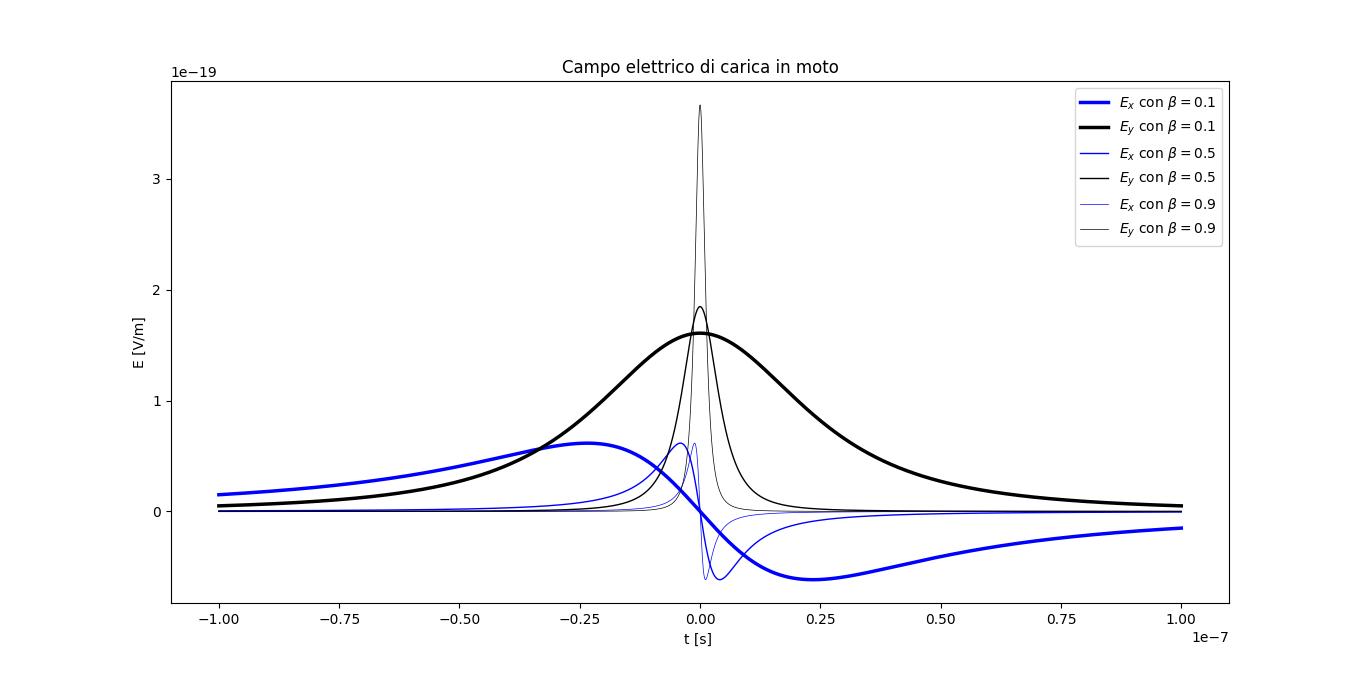
\includegraphics[width=0.8\textwidth]{immagini/carica_in_moto.png}
	\caption{Campi elettrici generati da una carica in moto}
	\label{fig:campo_carica_moto}
\end{figure}
Da notare che il campo lungo $y$ diventa sempre più stretto e piccato all'aumentare di $\beta$ (di conseguenza anche il campo magnetico, soltanto che questo è rifotto di un fattore $\beta$).

\subsection[]{Scrivere in forma covariante l'equazione del moto di una carica in un campo elettromagnetico esterno ("quadri-forza di Lorentz").}
\label{sec:3.b.7}
Analizziamo il caso di una particella puntiforme, l'equazione relativistica (tridimensionale) del moto è: \[
	\frac{\mbox{d} \bs{p}}{\mbox{d} t} = e\left( \bs{E}+ \frac{\bs{v}}{c}\wedge \bs{B} \right) 
.\] 
Nella quale l'impulso spaziale è $\bs{p}=m\gamma \bs{v}$.\\
È quindi ragionevole pensare che si debba sfruttare il 4-impulso $p^{\mu}=m u^{\mu}$ con $u^{\mu}=\gamma\left( c, \bs{v} \right)$, ed il tensore dei campi gia introdotto nelle domande precedenti, ovvero l'entità che contiene tutte le informazioni necessarie dei campi e che viene da un formalismo covariante. Per procedere si cerca quindi una equazione della forma:
\[
	\frac{\mbox{d} p^{\mu}}{\mbox{d} \tau}= N F^{\mu\nu} u_{\nu} 
.\]
Cercando una normalizzazione $N$ ragionando sulle dimensioni: per trarre una forza dall'espressione di destra ci serve una carica a moltiplicare ed una velocità a dividere, si prova ad utilizzare $\frac{e}{c}$. Si prova quindi componente per componente:
\begin{align*}
	F^{0i}u_{i}=& -E_{i}\cdot \left( -\gamma v_{i} \right) =\gamma \bs{E}\cdot \bs{v}\\
	F^{i\alpha}u_{\alpha}=&F^{i 0}u_0+F^{ij}u_{j}=E_{i}c\gamma-\epsilon_{ijk}B_{k}\left( -\gamma v_{j} \right) =\\
	=& c\gamma\left(\bs{E}+\frac{\bs{v}}{c}\wedge \bs{B}   \right) 
.\end{align*}
Considerando il fatto che 
\[
	dt= \gamma d\tau
\]
si ha che li componenti spaziali (le seconde calcolate) danno proprio l'equazione del moto.\\
Considerando invece che $P^{\mu}=\left(\varepsilon /c, \bs{p} \right)$ si ha che la componente temporale rappresenta il teorema delle forze vive:
\[
	\frac{\mbox{d} \varepsilon}{\mbox{d} t} = e \bs{E}\cdot \bs{v}	
.\] 


\subsection[]{Dimostrare che la forza di reazione radiativa è: 
\[
	\bs{F}_{\text{rad}}=\frac{2q^2}{3c^3}\dot{\bs{a}}=z^2m_e \tau_e \dot{\bs{a}} \quad \quad \text{con } \tau_e=\frac{2r_{e}}{3c}=\left(6.2\cdot 10^{-24}\right)
.\]
Indicare inoltre il campo di applicazione di quest'ultima.
}\label{sec:3.b.8}
La dimostrazione euristica e non relativistica è stata affrontata nella \hyperref[subsec: 2.a.15]{Domanda 2.a.15} insieme ai campi di applicazione (moto periodico). 

\subsection[]{Dare la definizione del "tensore energia-impulso" del campo elettromagnetico e scrivere la sua relazione con la "densità di forza di Lorentz".}
\label{sec:3.b.9}
Il tensore energia impulso è definito come:
\[
	\Theta^{\mu\nu}=\frac{1}{4\pi}\left( F^{\mu\alpha}F^{\nu}_{\alpha}- \frac{1}{4}\eta^{\mu\nu}F^{\alpha\beta}F_{\alpha\beta} \right) 
.\] 
Dove $\eta^{\mu\nu}$ è il tensore metrico diag$\left( 1,-1,-1,-1 \right)$.\\
Per inquadrarlo meglio lo si può vedere sotto forma di matrice: 
\[
	 \Theta= 
	 \left(
		 \begin{array}{c|ccc}
			 u_{\text{em}} 	& 		&	\bs{S}  	&	\\   
		 	\hline	 
					&		&  			&	\\
		 	\bs{S} 		&  		&  	-T_{\text{Maxwell}}		& 	\\
		 	 		&  		&  			& 	\\
		 \end{array}
	 \right) 
.\] 

Tale tensore è legato alla densità di forza di Lorentz da:
\[
	\partial_{\mu}\Theta^{\mu\nu}+f^{\nu}=0
.\] 
Dove la densità di forza di Lorentz ricordiamo essere: \[
	f^{\nu}=\frac{1}{c}F^{\mu\nu}j_{\nu}=\left( \frac{\bs{j}\bs{E}}{c}, \rho \bs{E}+\frac{1}{c} \bs{j}\wedge \bs{B}  \right) 
.\] \label{eq:conservazioni-relativita} 
\subsection[]{Dire come si generalizzano i teoremi di conservazione dell'energia e dell'impulso a situazioni in cui sia presente un campo elettromagnetico.}
\label{sec:3.b.10}
Nel caso dell'energia si ha (CGS):
\[
	\frac{1}{8\pi}\frac{\partial }{\partial t} \left( E^2+B^2 \right) + \frac{c}{4\pi}\nabla\left( \bs{E}\wedge \bs{B} \right) = - \bs{E}\cdot \bs{j}
.\] 
Nel caso dell'impulso invece: \[
	\frac{1}{4\pi}\frac{\partial}{\partial t}\left(\bs{E}\wedge\bs{B}\right)+\nabla\cdot T=-\left(\rho\bs{E}+\frac{\bs{j}}{c}\wedge \bs{B}\right) 
.\]
Con T tensore degli stress di Maxwell.\\
Entrambe le equazioni sono generaliate al caso relativistico dalla \hyperref[eq:conservazioni-relativita]{Equazione} che lega la densità di forza di Lorentz al tensore energia impulso.

\subsection[]{Scrivere il tensore degli sforzi per un’onda e.m. piana che si propaga in una direzione definita come $\hat{n}$.}
\label{sec:3.b.11}
Il tensore degli stress è definito come:
\[
	T= \I u_{\text{em}} - \frac{1}{4\pi} \left( E \otimes E + B \otimes B\right) 
\]
Oppure con gli indici:
\[
	T^{ij}= \delta^{ij}u_{\text{em}} - \frac{1}{4\pi}\left( E^{i}E^{j}+ B^{i}B^{j} \right) 
\]
Con 
\[
	u_{\text{em}}=\frac{1}{8\pi}\left( E^2 + B^2 \right) = \frac{1}{8\pi}\left( E_{i}E_{i}+ B_{j}B_{j} \right)
.\]
Quindi con un'onda piana che propaga nella direzione $\hat{n}$ si ha sempre (con una opportuna rotazione del sistema di riferimento) che \[
	T^{ij}=n^{i}n^{j}u_{\text{em}}
.\] 
Per verificarlo basta scegliere il sistema di riferimento in cui l'onda piana propaga nella direzione $\hat{x}=\hat{n}$, in questo modo si ha:
\begin{align*}
	\bs{E}=&E_0 \hat{y} e^{ikx-i \omega t}\\
	\bs{B}=&E_0 \hat{z} e^{ikx-i\omega t}
.\end{align*}
Da cui segue immediatamente che \[
	T^{ij}= \delta^{ij} \frac{E_{i}E_{i}+B_{i}B_{i}}{8 pi} - \frac{1}{4\pi}\left(  E^{i}E^{j}+B^{i}B^{j}\right)
\]
Non ci scordiamo che $E_i$ è diverso da zero solo con $i=1$ (ovvero per la componente $y$), allo stesso modo  $B_i$ è diverso da zero solo con $i=2$. Questo comporta che il secondo termine (quello con il segno meno nella espressione sopra) non si annulla solo per il secondo ed il terzo elemento diagonale (yy e zz) in cui vale $u_{\text{em}}$, tuttavia in entrambi i casi questi vengono annullati dalla presenza del primo termine (che è anche esso diagonale).\\
Infatti, essendoci una $\delta$, il primo termine si collocherà nella matrice $T$ solo sugli elementi diagonali, portando in ognuno di essi lo stesso scalare $u_{\text{em}}$. \\
Se ne conclude che:
\[
	T^{ij}=  u_{\text{em}}n^{i}n^{j}
.\] 
Dove il prodotto scalare tra $n^{i}$ e $n^{j}$ è solo un modo compatto per esprimere la matrice che scriveremo tra poco.
\begin{align*}
	\hat{n}=
	\left( 
	\begin{array}{c}
		i=0 \implies 1\\
		i=1 \implies 0\\
		i=2 \implies 0
	\end{array}
	\right) 
.\end{align*}
Facendo scorrere gli indici e provando a combinarli si trova la forma matriciale di $T$ :
\[
	T=
	u_{\text{em}}
	\left(
	\begin{array}{ccc}
		1 & 0 & 0 \\   
		0 & 0 & 0 \\
		0 & 0 & 0 \\
	\end{array}
	\right)
.\] 
\subsection[]{Scrivere esplicitamente il 4-tensore impulso-energia per un’onda elettromagnetica piana monocromatica che si propaga lungo l’asse x con densita’ di energia $u_{\text{em}}$.}
\label{sec:3.b.12}
Utilizzando i risultati della domanda 3.b.9 e 3.b.11 possiamo dire che:
\[
\Theta=
\left(
\begin{array}{cccc}
	u_{\text{em}} & u_{\text{em}}  & 0 & 0 \\   
	u_{\text{em}} & -u_{\text{em}} & 0 & 0 \\
	0 & 0 & 0 & 0 \\
	0 & 0 & 0 & 0 \\
\end{array}
\right)
.\] 
Riconosciamo nella matrice 3x3 in basso a destra il tensore degli stress calcolato in precedenza con il segno cambiato, in alto a sinistra la densità di energia ed ai lati il vettore di Poynting con la densità di energia collocata nella direzione di propagazione.
\subsection[]{Ricavare l’espressione per i potenziali di Lienard-Wiechert ( $\phi$ ed A per una carica puntiforme in moto arbitrario) a partire dai potenziali ritardati.}
\label{sec:3.b.13}
Ricordiamo l'espressione dei potenziali ritardati:
\begin{align*}
	\varphi\left( \bs{r},t \right)=	& \int \frac{\rho\left( \bs{r}', t-\left| \bs{r}-\bs{r}' \right|/c \right) }{\left| \bs{r}-\bs{r}' \right| }d^3r'\\
					&\\
	\bs{A}\left( \bs{r},t \right)=	& \frac{1}{c}\int \frac{\bs{j}\left( \bs{r}', t-\left| \bs{r}-\bs{r}' \right|/c \right)}{\left| \bs{r}- \bs{r}' \right|} d^3r'
.\end{align*}
Sia Q una carica che si muove con la legge oraria $\bs{s}\left( t \right) $, le densità di carica e di corrente ad essa assoiate sono:
\begin{align*}
	\rho\left( \bs{r},t \right) =&q\delta^3\left( \bs{r}-\bs{s}\left( t \right) \right)\\
	\bs{j}\left( \bs{r},t \right) =&q \dot{\bs{s}}\left( t \right) \delta^3\left(\bs{r}-\bs{s}\left( t \right)   \right)
.\end{align*}
Il tempo ritardato è definito come al solito:
\[
	c\left( t- t' \right) = \left| \bs{r}-\bs{s}\left( t \right)  \right| 
.\] 
Si procede quindi al calcolo del potenziale scalare, il calcolo del potenziale vettore è del tutto analogo.
\[	
	\varphi\left( \bs{r},t \right)=	 q\int \frac{\delta^3\left( \bs{r}'-\bs{s}\left( t-\left| \bs{r}- \bs{r}' \right|/c \right)  \right)  }{\left| \bs{r}-\bs{r}' \right| }d^3r'\\
.\] 
Si può quindi utilizzare la prorietà della delta :
\[
	\int \delta\left( f\left( x \right)  \right) dx \ \stackrel{f\left( x \right) = y}{=} \ \int\delta\left( y \right) \frac{1}{\left| f' \right| }dy= \left. \frac{1}{\left| f' \right| }\right|_{f\left( x \right) =0}
.\] 
Ricordandoci che lo stiamo applicando ad un caso vettoriale, concentriamoci sul cambio di variabile (prima uguaglianza della relazione sopra) nel nostro integrale abbiamo:
\[
	f\left( \bs{r}' \right) = \bs{r}'- \bs{s}\left( t- \frac{\left| \bs{r}-\bs{r}' \right| }{c} \right) 
.\]
Nel calcolo della derivata consideriamo direttamente il fatto che, rimanendo una $\delta$ all'interno dell'integrale dopo il cambio di variabile, l'integrale verrà calcolato nei punti in cui la $\delta$ si annulla. Nel nostro caso si annulla in $\bs{r}' = \bs{s}\left( t' \right) $, quindi calcoleremo la derivata di $f$ direttamente nel punto di annullamento della $\delta$ rimanendo astratti nella formulazione dell'integrale. 
E necessario anche notare che la parametrizzazione
\[
\hat{t}=t-\frac{\left| \bs{r}-\bs{r}' \right| }{c}
\]
è tanto valida quanto quella del tempo ritardato, deriveremo rispetto a questo tempo applicando le regole di derivazione di funzioni composte:
\begin{align*}
	\left. f'\left( \bs{r}' \right)\right|_{\bs{r}'=\bs{s\left( t' \right) }} =& \left[ 1 - \frac{\partial \bs{s}\left( t- \frac{\left| \bs{r}-\bs{r}' \right| }{c} \right) }{\partial \left( t - \frac{\left| \bs{r}-\bs{r}' \right| }{c} \right) } \cdot  
			\frac{\partial}{\partial \bs{r}'} \left( t- \frac{\left| \bs{r}-\bs{r}' \right| }{c} \right) \right]_{\bs{r}'=\bs{s}\left( t' \right) } =\\
			=&\left[ 1 - \frac{\bs{v}\left( t-\frac{\left| \bs{r}-\bs{r}' \right| }{c} \right) }{c}\cdot \frac{\left( \bs{r}-\bs{r}' \right) }{\left| \bs{r}-\bs{r}' \right| }\right]_{\bs{r}'=\bs{s}\left( t' \right) } =\\
	=& 1-\bs{\beta}\cdot \hat{n}
.\end{align*}

Inoltre è necessario scrivere il denominatore dell'integranda in funzione della nuova variabile y, senza perdere di generalità possiamo scriverlo come :
\[
	\left| \bs{r}-\bs{r}' \right| = \left| \bs{r}-f^{-1}\left( y \right)  \right| 
.\] 
Detto ciò l'integrale diventa:
\[
	\varphi\left( \bs{r}, t \right) = q\int \frac{\delta\left( y \right)}{\left| \bs{r}-f^{-1}\left( y \right)  \right| } \frac{1}{\left| f'\left( y \right)  \right| }dy 
.\]
Applicando la $\delta$ esce dall'integrale un termine $f^{-1}\left( y=0 \right) $; non è necessario esplicitarlo, basta applicare nuovamente l'operatore di inversione per farlo tornare $\bs{r}'$ calcolato in $\bs{s}\left( t' \right) $. Si conclude quindi che:
\[
	\varphi\left( \bs{r}, t \right) = \left[\frac{q}{\left| \bs{r}-\bs{s}\left( t \right)  \right| \left( 1-\bs{\beta}\left( t \right) \cdot \hat{n} \right) }\right]_{t=t'}
.\] 
Analogamente possiamo ricavare il potenziale vettore:
\[
	\bs{A}\left( \bs{r}, t \right) =\left[\frac{q \bs{\beta\left( t \right) }}{\left| \bs{r}-\bs{s}\left( t \right)  \right| \left( 1-\bs{\beta}\left( t \right) \cdot \hat{n} \right) }\right]_{t=t'}
.\] 

\subsection[]{Calcolare la potenza totale irraggiata da una carica accelerata in moto non relativistico. Esprimere i risultati in MKSA e nelle unità “naturali”.}
\label{sec:3.b.14}
Il campo elettrico di una carica in zona di radiazione è (nell'approssimazione non relativistica):
\[
	\bs{E}_{\text{rad}}\left( \bs{x},t \right)= \frac{q}{c} \left[ \frac{\hat{n}\wedge \left[ \left( \hat{n}-\bs{\beta} \right) \wedge \dot{\bs{\beta}}  \right] }
	{\left( 1-\hat{n}\cdot \bs{\beta} \right) R}  \right]_{\text{rit}}  \approx \frac{q}{c}\left[ \frac{\hat{n}\wedge \left(\hat{n}\wedge \dot{\bs{\beta}}\right)}{R}\right]_{\text{rit}} 
\]
Essendo il campo $\bs{B}=\hat{n}\wedge \bs{E}$ dal calcolo del vettore di Poynting si conclude che (conto affrontato nella domanda \hyperref[sec:3.b.3]{Domanda 3.b.3}):
\[
	\frac{\mbox{d} P}{\mbox{d} \Omega} = \frac{q^2\left| \hat{n}\wedge \dot{\bs{\beta}}\right|^2}{4\pi c}
.\] 
Integrando sull'angolo solido si ottiene che (sistema di riferimento con coordinate sferiche):
\[
	P = \frac{2q^2\left| \dot{\bs{\beta}} \right|^2}{3c}
.\] 
In MKSA si ottiene:
\[
	P = \frac{q^2\left| \dot{\bs{\beta}} \right|^2}{6\pi\epsilon_0c}
.\] 

\subsection[]{Ricavare la formula di Larmor relativistica 
\[
	P=\frac{2q^2}{3c^3}\gamma^{6}\left( \left| \bs{a} \right| ^2 - \left| \bs{a}\wedge \bs{\beta}  \right| ^2 \right) 
.\] a partire dalla formula non relativistica ed utilizzando argomenti di invarianza relativistica.}
\label{sec:3.b.15}
La potenza deve essere un invariante relativistico. Infatti è definita dal rapporto tra un energia ed un tempo, entrambe prime componenenti di un quadrivettore e quindi entrambe trasformanti allo stesso modo (come un tempo).\\
Conviene allora sfruttare l'invariante $a^{\mu}a_{\mu}$, con $a^{\mu}$ quadriaccelerazione definita da:
\[
	a^{\mu}=
	\left( \quad
	\begin{array}{c}
		\gamma^{4}\bs{a}\cdot \bs{\beta}, \quad 
		\gamma^2 \bs{a}+\gamma^{4} \left( \bs{a}\cdot \bs{\beta} \right) \bs{\beta}
	\end{array}
	\quad \right)
.\] 
Possiamo provare a vedere se la quantità giusta è: \[
	P=-\frac{2}{3} \frac{q^2}{c^3}a^{\mu}a_{\mu}
.\] 
Che è un invariante di Lorentz e soprattutto coincide con la formula non relativistica. Proviamo a vedere se torna con il caso cercato:
\begin{align*}
	a^{\mu}a_{\mu}=&\gamma^{4}\left( \gamma^{4}\left( \bs{a}\cdot \bs{\beta} \right) ^2 - \left| \bs{a}+ \gamma^2\left( \bs{a}\cdot \bs{\beta} \right) \bs{\beta} \right| ^2 \right)=\\
	=& \gamma^{4}\left( \gamma^{4}\left( \bs{a}\cdot \bs{\beta} \right)^2-\gamma^{4}\left| \bs{\beta} \right|^2 \left( \bs{a}\cdot \bs{\beta} \right)^2 - \left| \bs{a} \right| ^2 - 2\gamma^2\left( \bs{a}\cdot \bs{\beta} \right) ^2   \right) =\\
	=& \gamma^{4}\left( -\gamma^2\left( \bs{a}\cdot \bs{\beta} \right)^2-\left| \bs{a} \right|^2 \right)=\\
	=& \gamma^{6}\left( \left| \bs{\beta} \right|^2\cdot  \left| \bs{a} \right|^2 - \left( \bs{a}\cdot \bs{\beta} \right)^2 - \left| \bs{a} \right|^2\right)=\\
	=& \gamma^{6}\left( \left| \bs{a}\wedge \bs{\beta}  \right|^2-\left| \bs{a} \right|^2 \right) 
.\end{align*}
Da cui se ne conclude che la quantità provata è quella giusta.

\subsection[]{Dimostrare che la radiazione di sincrotrone ha uno spettro di emissione con una frequenza “critica” $\omega_{u}\approx \omega_0\gamma^3$.}
\label{sec:3.b.16}
Per arrivare al risultato costruiamo geometricamente la situazione di osservazione:
\begin{figure}[ht]
    \centering
    \incfig{luce-sincrotrone}
    \caption{Schema di rilevamento della Luce di Sincrotrone}
    \label{fig:luce-sincrotrone}
\end{figure}
Alla posizione $R$ di Figura c'è un rilevatore di radiazione elettromagnetica, la circonferenza rappresentata è la traiettoria della particella nell'acceleratore. Si rappresentano gli istanti $t'_{1}$ e $t'_{2}$ in cui la radiazione (che può essere rilevata da $R$) viene emessa dalla sorgente. Se la radiazione emessa in tali istanti viene rilevata allora arriva al rivelatore rispettivamente agli istanti $t_{1}$ e $t_{2}$, questa notazione induce le relazioni:
\begin{align*}
	t_1 =& t'_{1}+ \frac{\Delta L + D}{c}\\
	t_2=& t'_{2}+ \frac{D}{c}=t'_{1}+ \frac{\Delta L}{V}+ \frac{D}{c}
.\end{align*}
Possiamo allora dare una stima del tempo in cui si osserva la radiazione come:
\begin{align*}
	\Delta t =& t_2-t_1 =\\
	=&\frac{\Delta L}{V}- \frac{\Delta L}{c}=\\
	=& \Delta L \left( \frac{1}{\beta c} - \frac{1}{c} \right) 
.\end{align*}
Adesso dobbiamo sfruttare il fatto che per particelle che viaggiano a velocità relativistiche $1 /\gamma \approx 1$, quindi l'angolo in figura taglierà un arco di circonferenza piccolo rispetto alle dimensioni dell'apparato. Quindi:
\begin{align*}
	\Delta L \approx \frac{2 \rho}{\gamma} \quad \implies \quad  \Delta t \approx \frac{2\rho}{\gamma}\left( \frac{1-\beta}{\beta c} \right) 
.\end{align*}
Infine moltiplicando e dividendo per $1+\beta$:
\[
	\Delta t = \frac{2 \rho}{\gamma \beta c} \left( \frac{1-\beta^2}{1+\beta} \right)\approx \frac{\rho}{c \gamma^3} 
.\] 
Logicamente se l'impulso dura $\Delta t$ significa che lo spettro angolare di radiazione si estende fino ad una frequenza critica:
\[
	\omega_{c} \sim \frac{1}{\Delta t} = \frac{c\gamma^3}{\rho}= \omega_0\gamma^3
.\] 

\subsection[]{Calcolare il fattore di forma elettromagnetico per una sfera uniformente carica di raggio a.}
\label{sec:3.b.17}
La sfera di raggio $a$ uniformemente carica avrà una distribusione di carica esprimibile come:
\begin{align*}
	\rho\left( \bs{r} \right) =
	\begin{cases}
	\ \frac{3Q}{4\pi a^3} \quad &\text{se} \quad \left| \bs{r} \right| < a  \\
	\ 0  \quad  &\text{se} \quad \left| \bs{r} \right| > a \\
	\end{cases} 
.\end{align*}
Per un dato valore di $q$ scegliamo delle coordinate polari aventi l'asse polare diretto lungo $q$ stesso, si calcola quindi il fattore di forma come:
\begin{align*}
	F\left( \bs{q} \right) 	&= \frac{\int \rho\left( \bs{r} \right) e^{-i \bs{q}\cdot \bs{r}}d^3r}{\int \rho\left( \bs{r} \right) d^3r} \\
			       	&= \frac{1}{Q}\int_{0}^{a}dr\int_{0}^{\pi}d\theta \int_{0}^{2\pi} d\phi \rho\left( r \right) e^{-irq\cos\theta} r^2 \sin\theta \\
			     	&=  \frac{2\pi}{Q}\int_0^a\int_{1}^{-1} \rho\left( r \right) e^{-irq\cos\theta} r^2 \left| d\cos\theta \right| dr=\\ 
				&= \frac{4\pi}{Q} \int_0^{a} \rho\left( r \right) r^2 \frac{\sin\left( qr \right) }{qr}dr= \\
				&= \frac{3}{a^3q}\int_0^{a} r \sin\left( qr \right) dr= \\
				&= \frac{3}{a^3} \left(- \frac{1}{q} r\cos\left( qr \right) + \frac{1}{q^2} \sin \left( qr \right)  \right)_{0}^{a}= \\
				&= 3\left( \frac{\sin\left( aq \right) }{\left( aq \right)^3 } -\frac{\cos\left( aq \right) }{\left( aq \right) ^2} \right)  
.\end{align*}
In quest'ultima si può notare che, grazie alla simmetria del sistema sotto rotazioni, $F\left( \bs{q} \right) = F\left( q \right) $
\subsection[]{Calcolare il fattore di forma per una supeficie sferica uniformente carica di raggio a. [nota: l'interno è vuoto]}
\label{sec:3.b.18}
In tal caso la densità di carica si può esprimere come:
\begin{align*}
	\rho\left( \bs{r} \right) =
	\begin{cases}
		\ 0 \quad \text{se} \quad  \left| \bs{r} \right| < a\\
		\ \frac{Q}{ 4 \pi a^2} \quad \text{se} \quad \left| \bs{r} \right| = a\\
		\ 0 \quad \text{se} \quad \left| \bs{r} \right| > a
	\end{cases}
.\end{align*}
Procedendo come sopra senza interare su $r$ si ottiene:
\[
	F\left( \bs{q} \right) = \frac{3\sin\left( aq \right) }{a^2q}
.\] 

\subsection[]{Calcolare la velocità di un elettrone [e successivamente di un protone] posto in una struttura acceleratrice che abbia: \\
	1) Campo elettrico longitudinale costante.\\ 
	2) Campo elettrico longitudinale oscillante.\\ 
Inserendo valori numerici ragionevoli, calcolare il tempo affinché la particella, partendo da ferma, raggiunga una energia pari al doppio della sua massa a riposo.}
\label{sec:3.b.19}
Supponiamo la struttura lineare, l'equazione di moto di una particella nel campo dell'acceleratore è:
\[
	\frac{\mbox{d} }{\mbox{d} t} \left( p_{x} \right) = qE \implies	\frac{\mbox{d} }{\mbox{d} t}\left( \gamma \beta \right)  = \frac{qE}{mc}
.\] 
\paragraph{Campo elettrico costante}%

Nel caso di campo costante l'equazione si risolve con:
\[
	\gamma \beta = \frac{qE}{mc}\cdot  t = \frac{t}{\tau}
.\] 
Per trovare la velocità (quindi $\beta$) dobbiamo esplicitare $\gamma$ nella precedente:
\[
	\frac{\beta^2}{1-\beta^2}= \frac{t^2}{\tau^2}\implies \beta=\frac{t}{\sqrt{t^2+\tau^2} }
.\] 
Da cui l'energia:
\[
	E= mc^2\gamma= mc^2\sqrt{1+\frac{t^2}{\tau^2}} 
.\] 
Ne segue che per avere una energia che sia il doppio di quella a riposo bisogna imporre:
\begin{align*}
	2=\sqrt{1+\frac{\Delta t^2}{\tau^2}} \implies \Delta t = \sqrt{3}\tau \approx 
	\begin{cases}
		10^{-11} & \text{per l'elettrone}\\
		10^{-7} &  \text{per il protone}
	\end{cases} 
.\end{align*}
Nella stima numerica è stato preso il valore tipico di campo elettrico per un acceleratore lineare di $50$ MeV/m.
\paragraph{Campo elettrico oscillante}%
Gli acceleratori costruiti con questo metodo accelerano le particelle solo nel semiperiodo in cui il campo elettrico è diretto nella direzione in cui è attesa la accelerazione, per far ciò si alternano zone in cui il campo è presente a zone in cui invece non lo è.
\begin{figure}[H]
	\centering
	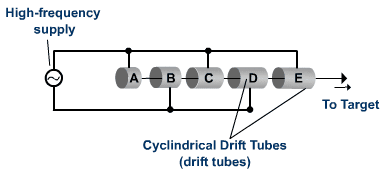
\includegraphics[width=0.4\textwidth]{immagini/drift-tube.png}
	\caption{Drift Tube in un acceleratore lineare}
	\label{fig:Drift Tube}
\end{figure}
Prendiamo adesso un campo elettrico del tipo :
\[
	E= E_0\sin\left( \frac{\pi t}{\tau'} \right) 
.\] 
Non possiamo più applicare il metodo utilizzato sopra, potremmo in qualche modo cercare di discretizzare il problema mediando l'equazione del moto su un semiperiodo (per i motivi spiegati all'inizio), la variabile diventa allora il tempo impiegato a fare un semiperiodo $\tau'$:
\[
	\Delta \left( \beta\gamma \right) = \frac{qE_0}{mc}\int_0^{\tau'} \sin \left( \frac{\pi t}{\tau} \right) dt = \frac{2qE_0\tau'}{\pi mc}
.\] 
Quindi ogni volta che la particella attraversa un Drift tube subisce una variazione di $\gamma\beta$ come quella scritta sopra.
Se parametrizziamo il modulo del campo elettrico iniziale come:
\[
	E_0 \rightarrow \frac{2E_0}{\pi} = E'_0
.\] 
ci si accorge che il risultato non è tanto differente da quello incontrato nel caso di campo costante (ipotizziamo sempre che la particella sia idealmente ferma nel momento dell'accenzione del campo).
\[
	\Delta \gamma\beta = \gamma_{\text{fin}}\beta_{\text{fin}}=\frac{qE'_0}{mc}\tau'=\frac{\tau'}{\hat{\tau}}
.\] 
con $\hat{\tau}=\frac{qE'_0}{mc}$.\\
Notiamo che se vogliamo la quantità $\gamma\beta$ dopo che la particella ha attraversato $n$ Drift Tube basta sommare $n$ volte la quantità $\tau' /\hat{\tau}$.
calcoliamo la velocità della particella all'uscita dell'ennesimo Drift Tube sfruttando il calcolo effettuato in precedenza:
\[
	\beta = \frac{n \tau'}{\sqrt{\hat{\tau}^2 + n^2 \tau'^2} }
.\] 
E in modo analogo l'energia:
\[
	E = mc^2\sqrt{1+\frac{n^2\tau'^2}{\hat{\tau}^2}} 
.\] 
La ricerca del tempo in cui la particella raggiunge il doppio dell'energia a riposo richiede questa volta una piccola considerazione aggiuntiva: per ogni semi periodo trascorso in presenza del campo elettrico ve ne è uno trascorso all'esterno dei Drift Tube. Dobbiamo quindi aggiungere al tempo necessario all'interno dei drift tube (sempre in termini di semi periodi) il tempo trascorso all'esterno senza campo elettrico ed a velocità costante.
\[
	n\tau' + n\tau' = \sqrt{3}\hat{\tau} \implies 2n\tau' = \sqrt{3} \hat{\tau}
.\] 
E chiamando $2\tau'= T$ il periodo di oscillazione si ha:
\[
	nT = \sqrt{3}\frac{2qE_0}{\pi mc}
.\] 
I tempi in cui si riesce a raddoppiare l'energia hanno la stessa espressione  (fattore $\frac{2}{\pi}$ a parte), visto che le tensioni che si riesce a raggiungere nei due casi sono simili anche il valore numerico di tali tempi non differisce di molto.

\subsection[]{A partire dai campi ritardati, dimostrare che 
\[
	\frac{\mbox{d} P}{\mbox{d} \Omega} = \frac{q^2\left| \bs{a} \right|^2\sin^2\theta }{16\pi^2\epsilon_0c^3\left( 1-\beta\cos\theta \right)^5 }
.\] è la potenza (MKSA) irraggiata da una carica accelerata in un moto rettilineo.}
\label{sec:3.b.20}
I campi ritardati citati nel testo sono:
\[
	\bs{E}\left( \bs{x},t \right)= \frac{q}{c} \left[ \frac{\hat{n}\wedge \left[ \left( \hat{n}-\bs{\beta} \right) \wedge \dot{\bs{\beta}}  \right] }
	{\left( 1-\hat{n}\cdot \bs{\beta} \right)^3 R}  \right]_{\text{rit}} 
.\] 
Nel caso affrontato essendo il moto rettilineo velocità ed accelerazione sono parallele, quindi:
\[
	\bs{E}\left( \bs{x},t \right)= \frac{q}{c} \left[ \frac{\hat{n}\wedge \left( \hat{n}  \wedge \dot{\bs{\beta}}  \right) }
	{\left( 1-\hat{n}\cdot \bs{\beta} \right)^3 R}  \right]_{\text{rit}} 
.\] 
Come sempre si può ricavare il vettore di Poynting utilizzando il modulo quadro del campo elettrico:
\[
	\bs{S\left( t \right) }= \frac{c}{4 \pi }\left| \bs{E} \right|^2_{\text{rit}} \hat{n} = 
	\frac{q^2}{4 \pi c}\left|  \frac{\hat{n}\wedge \left( \hat{n}  \wedge \dot{\bs{\beta}}  \right) }{\left( 1-\hat{n}\cdot \bs{\beta} \right)^3 R^2} \right|^2_{\text{rit}} \hat{n}
.\] 
In questo modo si ha il vettore di Poynting parametrizzato per unità di tempo, infatti con questo potremmo calcolare l'energia che attraversa l'elemento infinitesimo di area come:
\[
	W= \int_{-\infty}^{\infty} dt \bs{S}\left( t \right) \cdot \hat{n}
.\] 
Se nell'integrale facciamo il cambio di variabile
\[
	W= \int_{-\infty}^{\infty} dt' \frac{dt}{dt'} \bs{S}\left( t\left( t' \right)  \right) \cdot \hat{n}
.\]
Possiamo ridefinire l'integranda come la potenza irraggiata istantaneamente dalla particella
\[
	\frac{\mbox{d} W}{\mbox{d} t'}= \frac{dt}{dt'} \bs{S}\left( t\left( t' \right)  \right) \cdot \hat{n} 
.\] 
calcolata al tempo in cui la radiazione viene emessa e non al tempo ritardato, ovvero esattamente quella che vogliamo considerare. 
Lo Jacobiano di questo cambio di variabile è (calcolato nella \hyperref[sec:3.b.1]{Domanda 3.b.1}):
\[
	\frac{dt}{dt_{\text{rit}}}= 1- \hat{n}\cdot \bs{\beta}
.\] 
Quindi la potenza irraggiata per unità di angolo solido tornando in MKSA è (come già visto nella \hyperref[sec:3.b.3]{Domanda 3.b.3}): 
\begin{align*}
	\frac{\mbox{d} P}{\mbox{d} \Omega} &= \left| \bs{S} \right| R^2 =\\
	&=  \frac{q^2}{16\pi^2\epsilon_0 c} \left|  \frac{\hat{n}\wedge \left( \hat{n}  \wedge \dot{\bs{\beta}}  \right) }{\left( 1-\hat{n}\cdot \bs{\beta} \right)^3 } \right|^2\left( 1-\hat{n}\cdot \bs{\beta} \right) =\\
	&=  \frac{q^2}{16\pi^2\epsilon_0 c} \frac{\left| \hat{n}\wedge \left( \hat{n}\wedge \dot{\bs{\beta}}  \right)   \right|^2 }{\left( 1-\hat{n}\cdot \bs{\beta} \right)^{5} }
.\end{align*}
Per concludere la dimostrazione manca adesso il sistema di riferimento in coordinate sferiche, facendo riferimento alla seguente figura
\begin{figure}[H]
    \centering
    \incfig{sistema-potenza-relativistica}
    \caption{Sistema di riferimento per una carica accelerata linearmente.}
    \label{fig:sistema-potenza-relativistica}
\end{figure}
è facile concludere l'uguaglianza tra la formula trovata in forma vettoriale sopra e quella richesta nel testo.



\subsection[]{Calcolare l’energia persa in una rivoluzione per una carica in moto uniforme su una circonferenza (acceleratore circolare). Calcolare la frazione di energia persa
in un giro rispetto alla sua energia cinetica, effettuando una valutazione numerica, nel caso di elettroni a LEP (energia 50 GeV, raggio 4km) o protoni ad LHC (energia 7 TeV, raggio ~4km). Nota: utilizzare la formula di Larmor in GCS:
\[
	P=\frac{2q^2}{3c^3}\gamma^{6}\left( \left| \bs{a} \right| ^2 - \left| \bs{a}\wedge \bs{\beta}  \right| ^2 \right) 
.\] }
\label{sec:3.b.21}
Sia $a$ l'accelerazione radiale della particella nel suo moto, $R$ il raggio di curvatura totale e $R_{B}$ il raggio di curvatura nel tratto esclusivamemnte composto da zone con campo magnetico (quelle adibite a curvare).\\
Nel caso di moto uniforme su una circonferenza abbiamo visto nella \hyperref[sec:3.a.21]{Domanda 3.a.21} che la formula di Larmor si può riscrivere come (CGS):
\[
	P = \frac{2\gamma^4\beta^4}{3}\frac{q^2c}{R_{B}^2}
.\] 
O anche, per effettuare stime numeriche, in MKSA:
\[
	P = \frac{\gamma^4\beta^4}{6\pi\epsilon_0}\frac{q^2c}{R_{B}^2}
.\] 
Per una stima della energia persa al giro in irraggiamento dobbiamo considerare solo le zone in cui vi è accelerazione di carica, quindi le zone di curvatura in cui vi è un campo magnetico. Tale tempo, se la particella viaggia a velocità costante è:
\[
	T_{B}= \frac{2\pi R_{B}}{\beta c}
.\] 
Quindi la variazione di energia sul giro (aggiungiamo e togliamo termini per renderla più interpretabile):
\begin{align*}
	\Delta E &= P\cdot T_{B}=\\
	&=  \frac{\gamma^4\beta^4}{6\pi\epsilon_0}\frac{q^2c}{R_{B}^2}\frac{2\pi R_{B}}{\beta c}=\\
	&=  \frac{4\pi }{3}\frac{q^2}{4\pi\epsilon_0m_e c^2} m_ec^2\frac{\beta^3\gamma^4}{R_B}\\
	&= \frac{4\pi}{3}\left( \frac{r_e}{R_B} \right) m_e c^2\beta^3\gamma^4 \\
\end{align*}	
Possiamo quindi già fare una prima stima numerica lasciando liberi i parametri che variano nei due casi:
\[
\Delta E \approx 4 \cdot 2.8 \text{ [fm]}\cdot 0.51 \text{ [MeV]} \frac{\beta^3\gamma^4}{R_B} \approx 5.6 \text{ [fm]} \cdot \text{[MeV]} \frac{\beta^3\gamma^4}{R_B} 
.\] 
Con i dati del testo possiamo calcolare le quantità necessarie alla stima di $\gamma$ e $\beta$:
\begin{align*}
	&\gamma = \frac{E}{mc^2}  &\beta = \sqrt{1- \frac{1}{\gamma^2}} 
.\end{align*}

\paragraph{Acceleratore LEP}%
In tal caso si ha $\gamma=(50 \cdot 10^{3}) / 0.51 \approx 10^5$, $\beta \approx 1$ quindi:
\begin{align*}
	& \Delta E \approx \frac{5.6 \cdot 10^{-15}}{4 \cdot 10^{3}} \cdot 10^{20}\text{ [MeV]}=1.4 \cdot 10^{2} \frac{\text{ [MeV]} }{\text{giro}} = 
	0.14 \frac{\text{ [GeV]} }{\text{giro}}
.\end{align*}
Che da quindi una frazione di energia persa per giro di $\Delta E / E \approx 0.3 \%$
\paragraph{Acceleratore LHC}%
La massa del protone fa la differenza su $\gamma$ e su $\beta$ :
\begin{align*}
	&\gamma = \frac{7 \cdot 10^{6} \text{ [MeV]}}{9.383 \cdot 10^{2}  \text{ [MeV]}}\approx 7.5 \cdot 10^{3} \\
	&\beta \approx \sqrt{1- 10^{-8}}\approx 1 
.\end{align*}
Per l'energia quindi:
\begin{align*}
	& \Delta E \approx \frac{5.6 \cdot 10^{-15} }{4 \cdot 10^{3} } \left( 7.5 \cdot 10^{3}  \right) ^4 \text{ [MeV]} \sim \text{ [eV]}  
.\end{align*}
Da cui si deduce che la frazione di energia persa per irraggiamento nel caso di protoni è pressochè nulla.

\subsection[]{Calcolare la potenza emessa in funzione dell’angolo per una carica oscillante armonicamente in linea retta (termine di dipolo elettrico)}
\label{sec:3.b.22}
Potremmo riallacciarci al campo di radiazione del dipolo sempre passando per i campi di radiazione di Lineard-Wiechert nell'approssimazione non relativistica:
\begin{align*}
\bs{E}_{\text{rad}}\left(\bs{x},t\right) 	&\approx\frac{q}{c}\left[\frac{\hat{n}\wedge\left(\hat{n}\wedge\dot{\bs{\beta}}\right)}{R}\right]_{\text{rit}} \\
						&= \frac{q}{c^2R} \left[ \left( \ddot{\bs{x}}\wedge \hat{n} \right)\wedge \hat{n}\right]_{\text{rit}}  \\
						&= \frac{1}{c^2R} \left( \left[ \ddot{\bs{p}} \right]_{\text{rit}}\wedge \hat{n}\right)\wedge \hat{n}
.\end{align*}
Dove $\bs{p}$ è il momento di dipolo oscillante del tipo: $\bs{p} = qx_0e^{i \omega t}\hat{x}$, preso in questo caso (a titolo di esempio) nella direzione $\hat{x}$.\\
Abbiamo visto in precedenza (\hyperref[sec:3.b.3]{Domanda 3.b.3}) che la potenza irraggiata per unità di angolo solido si può esprimere come:
\[
	\frac{\mbox{d} P}{\mbox{d} \Omega}  = R^2\left| \bs{S} \right| = R^2 \frac{c}{4\pi} \left| \bs{E}_{\text{rad}} \right|^2 
.\] 
Chiamando quindi $\theta$ l'angolo tra la direzione di oscillazione $\hat{x}$ e la direzione di osservazione $\hat{n}$ possiamo eesprimere i prodotti vettoriali in funzione di tale angolo, inoltre la doppia derivata fa scendere un fattore $\omega^2$, se ne conclude che: 
\[
	\frac{\mbox{d} P}{\mbox{d} \Omega} = \frac{\left| \bs{p} \right|^2 \omega^4}{4\pi c^3} \sin^2\theta
.\] 

\subsection[]{Calcolare, a partire dalla formula di Larmor relativistica, la potenza totale dissipata in un acceleratore lineare in funzione di $\frac{\mbox{d} \bs{p}}{\mbox{d} t}$ oppure di $\frac{\mbox{d} E}{\mbox{d} x}$ (energia fornita per unita’ di lunghezza). Dimostrare che la frazione di energia persa nell’accelerazione e’ trascurabile, fornendo adeguati valori numerici nel caso di accelerazione di elettroni o protoni.}
\label{sec:3.b.23}
Come visto nella \hyperref[sec:3.a.21]{Domanda 3.a.21} la potenza dissipata per irraggiamento in un acceleratore lineare è:
\[
	P = \frac{q^2\gamma^6}{6\pi\epsilon_0}\left| \bs{a} \right|^2=\frac{q^2}{6\pi\epsilon_0m^2}\left| \frac{\mbox{d} \bs{p}}{\mbox{d} t}  \right|^2
.\] 
Infatti per la componente spaziale del quadrimpulso si ha:
\begin{align*}
	\frac{\mbox{d} p}{\mbox{d} t} 	&= \frac{\mbox{d} mv\gamma}{\mbox{d} t} =\\
				      	&= m a \gamma + m v \frac{\mbox{d} \gamma}{\mbox{d} t} =\\
					&= ma\gamma + ma\beta^2\gamma^3=\\
					&= ma\gamma^3 
.\end{align*}
Inoltre siamo andati subito in una dimensione essendo il moto unidimensionale.
Se la volessimo in funzione della variazione lineare di energia potremmo sfruttare la relazione:
\begin{align*}
	c \frac{\mbox{d} p}{\mbox{d} t} &= \frac{\mbox{d} }{\mbox{d} t}\sqrt{E^2-m^2c^4} =\\
	&= \frac{2E}{2\sqrt{E^2-m^2c^4} }\frac{\mbox{d} E}{\mbox{d} t}=  \\
	&= \frac{E}{cp}\frac{\mbox{d} E}{\mbox{d} t} = \\
	&= \frac{mc^2\gamma}{mv\gamma c}\frac{\mbox{d} E}{\mbox{d} t} = \\
	&= \frac{1}{\beta}\frac{\mbox{d} E}{\mbox{d} t} = \\
	&= c \frac{\mbox{d} E}{\mbox{d} x}  
.\end{align*}
Quindi si otterrebbe il medesimo risultato.\\
L'uguaglianza tra le due variazioni ci è utile invece per calcolare $f_{\text{rad}}$: la frazione di energia persa rispetto all'incremento di energia:
\begin{align*}
	f_{\text{rad}}	&= \frac{P}{\frac{\mbox{d} E}{\mbox{d} t} }=\\
		      	&= \frac{q^2}{6\pi\epsilon_0 c^3m^2}\left( \frac{\mbox{d} p}{\mbox{d} t} \right)^2 \frac{1}{v \frac{\mbox{d} E}{\mbox{d} x} }=  \\
			&= \frac{2}{3\beta} \frac{r_e \left( \frac{\mbox{d} E}{\mbox{d} x}  \right) }{mc^2} 
.\end{align*}
Si vede che questa è trascurabile sempre, infatti in una distanza dell'ordine dei fm non si riescono ad ottenere variazioni di energia dell'ordine di  $mc^2$.\\
La domanda del testo era invece la frazione di energia persa $\hat{f}$, la calcoliamo sempre a partire dalla formula di Larmor:
\[
	P= \frac{q^2}{6\epsilon_0c^3}\gamma^6 a^2= 
	 \frac{q^2}{6\pi\epsilon_0c^3}\frac{1}{m^2}\left( \frac{\mbox{d} p}{\mbox{d} t}  \right)^2 
\]
sia $E_0$ il modulo del campo elettrico applicato,  si ha sempre dall'equazione di moto:
\[
	\frac{\mbox{d} p}{\mbox{d} t} = qE_0
.\] 
Introducendo questa nella potenza irraggiata:
\[
	P= \frac{q^4E^2_0}{6\pi\epsilon_0m^2c^3}
.\] 
Il calcolo da effettuare per ottenere $\hat{f}$ è:
\[
	\hat{f}= \frac{P\cdot t_f}{E_f}
.\] 
Dove $t_f$ è il tempo necessario a raggiungere l'energia finale $E_f$. Si risolve se $t_f$ è lineare in $E_f $, calcoliamo questo tempo seguendo la linea di quanto fatto nella \hyperref[sec:3.b.19]{Domanda 3.b.19}:
\[
	\gamma_f=\sqrt{1+\left( \frac{t_f}{\tau} \right)^2 } \implies t_f =
	\tau\sqrt{\gamma^2_f-1} \approx \tau \cdot \gamma_f = \frac{mc}{qE_0}\cdot \frac{E_f}{mc^2}= \frac{E_f}{qE_0 c}
.\] 
Otteniamo quindi che:
\[
	\hat{f} = \frac{q^4}{6\pi \epsilon_0m^2c^2}\frac{E_0}{q}=\frac{E_0}{E_{\text{crit}}}
.\] 
Concentriamoci su $E_{\text{crit}}$, nel caso di elettroni:
\[
	E_{\text{crit}}=q \frac{6\pi\epsilon_0m^2c^4}{q^4}= \frac{3}{2}\frac{q}{4\pi\epsilon_0 r_e^2} \approx 2.7 \cdot 10^{20} \ \frac{\text{[V]}}{\text{[m]}}
.\] 
Quindi non c'è speranza, si raggiungono al massimo i MV/m: trascurabile.\\
Nel caso di protoni invece non occorre nemmeno fare il conto: basta guardare l'espressione di $\hat{f}$, dipende inversamente dalla massa, se è trascurabile per gli elettroni lo è anche per i protoni.


\subsection[]{Calcolare la lunghezza d’onda critica della radiazione di sincrotrone (elettroni) nei casi seguenti: \\
i) energia=50GeV, raggio=4km; \\
ii) energia=5GeV, raggio=30m}
\label{sec:3.b.24}
La frequenza critica è stata calcolata nella \hyperref[sec:3.b.16]{Domanda 3.b.16}, la lunghezza d'onda critica che ne deriva è:
\[
	\lambda_c = \frac{2\pi c}{\omega_c} = \frac{2\pi\rho}{\gamma^3} 
.\] 
con $\rho$ raggio dell'acceleratore.
\paragraph{Caso i)}    $\gamma\approx 10^5 \implies \lambda_{c}\approx 0.25 \text{ A}^o$
\paragraph{Caso ii)}	$\gamma\approx 10^4 \implies \lambda_{c}\approx 1.8 \text{ A}^o $


\subsection[]{Enunciare il teorema ottico e spiegarne il significato fisico nel caso di radiazione elettromagnetica su un ostacolo opaco.}
\label{sec:3.b.25}
Si consideri un'onda elettromagnetica $\bs{E}_{in}= \bs{E}_{0}e^{-i\left( \omega t - kz \right) }$ incidente su un bersaglio opaco ortogonalmente. Tale "interazione" produce una onda sferica rifratta che può essere scritta come:
\[
	\bs{E}_s= \frac{e^{-i\left( \omega t - kr \right) }}{r}\bs{f}\left( \bs{k} \right) 
.\] 
Dove $\bs{f}\left( \bs{k} \right) $ è l'ampiezza di scattering: racchiude tutta la dinamica del processo diffrattivo.\\
Si ha che la potenza dissipata in tutto il processo di scattering è:
\[
	P_{\text{diss}}= \frac{c}{2k} \text{Im}\left[ \bs{E}^*_{0}\cdot \bs{f}\left( k \hat{z} \right)   \right] 
.\] 
Che è l'enunciato del teorema ottico.

\subsection[]{Come si ricava la sezione d'urto differenziale Rayleigh a partire dalla sezione d'urto Thomson ?}
\label{sec:3.b.26}
Nello scattering Thompson si ha che, per un fotone che incide su un elettrone:
\[
	\left.\frac{\mbox{d} \sigma_{\text{el}}}{\mbox{d} \Omega}\right|_{\text{el}} =  \frac{r^2_e\omega^4}{\left( \omega^2_0-\omega^2 \right)^2 + \omega^2\Gamma^2_{\text{tot}}\left( \omega \right)} \sin^2\alpha
.\] 
Con $\alpha$ angolo tra la direzione di polarizzazione del campo e direzione di osservazione. Per il resto della notazione facciamo riferimento alle domande \hyperref[subsec: 2.a.15]{2.a.15} e \hyperref[subsec: 2.a.16]{2.a.16}. \\
Lo scattering Rayleigh serve invece nel caso di più centri scatteranti, come ad esempio un'onda incidente su un atomo, in tal caso è necessario introdurre nel calcolo della potenza irraggiata l'effetto della possibile interferenza tra i campi generati dai vari elettroni.\\
A questo scopo nasce il fattore di forma, tiene di conto di tali interferenze, in modo tale che se avessimo una distribuzione $\rho$ di carica con $\int \rho\left( \bs{r}\right)d^3r=Q$ il campo generato da questa non sarebbe altro che il campo di una carica puntiforme Q moltiplicato per $F\left( \bs{q} \right) $ della distribuzione.\\
Risulta quindi chiaro che l'unica correzione da aggiungere allo scattering dell'elettrone singolo è proprio il modulo quadro di questo fattore moltiplicato per il numero di elettroni presenti nell'atomo: lo scattering Rayleigh risulta:
\[
	\frac{\mbox{d} \sigma_{\text{el}}}{\mbox{d} \Omega} = \left.\frac{\mbox{d} \sigma_{\text{el}}}{\mbox{d} \Omega}  \right|_{\text{el}}\left| ZF\left( \bs{q} \right)  \right| ^2
.\] 




